% Información para el motor (arara). Compilar en LuaLaTeX o XeLaTeX sólamente.

%arara: lualatex: {
%arara: --> interaction: nonstopmode,
%arara: --> options: ['-file-line-error'],
%arara: --> shell: yes,
%arara: --> synctex: yes,
%arara: --> }
%arara: bib2gls if found("aux", "glsxtr@resource")
%arara: makeglossaries if found("aux", "@istfilename")
%arara: makeindex

\documentclass[letterpaper,twoside]{article}

%%%%%%% VARIABLES ESTÁTICAS %%%%%%%
% Aqui se definen las variables para diferentes procedimientos.
% Verificar que las unidades coincidan si se deciden cambiar.

\newcommand{\defglo}[1]{\item[{\bfseries \glsname{#1}}] \glsdesc{#1}} % Define un comando para dar un item en un entorno de descripción para una palabra definida en el glosario
% \includeonly{src/PSA-2.19.tex,src/PSA-Gloss.tex}
\newcommand{\TipoID}{TEMP} % Definirlo como: PRO, PROG, ToC, G, L, CE, CI, I, etc.
\newcommand{\Prog}{TEMP}
\newcommand{\ProgTitulo}{TEMP}

\newcommand{\ie}{\emph{i.e.}}
\newcommand{\eg}{\emph{e.g.}}

%%%%%%%%%%%%%%%% Formularios %%%%%%%%%%%%%%%%
\newcommand{\IdFormAACC}{F-OP-40}

\newcommand{\BitES}{Bitácora de entradas y salidas --- Clientes (F-AD-1)}
\newcommand{\BitULl}{Bitácora de uso de llaves (F-AC-1)}
\newcommand{\BitVig}{Bitácora de vigilancia (F-AC-2)}
\newcommand{\Fpap}{Papeleta (F-AC-3)}
\newcommand{\Oent}{Orden de entrada (F-AC-4)}
\newcommand{\Osal}{Orden de salida (F-AC-5)}
\newcommand{\LayES}{Layout de carga o descarga (F-AC-6)}
\newcommand{\BitClor}{Bitácora de cloración de agua (F-AC-7)}
\newcommand{\BitTap}{Bitácora de concentración de tapete sanitario (F-AC-8)}
\newcommand{\BitUQ}{Bitácora de uso de productos químicos (F-AC-9)}
\newcommand{\BitLAd}{Bitácora de limpieza de aduana sanitaria (F-AC-10)}
\newcommand{\BitLOf}{Bitácora de limpieza de oficinas (F-AC-11)}
\newcommand{\BitLEx}{Bitácora de limpieza de exteriores (F-AC-12)}
\newcommand{\BitBPH}{Bitácora de cumplimiento de BPH (F-HyS-1)}
\newcommand{\BitCAP}{Bitácora de consumo de agua potable (F-HyS-2)}
\newcommand{\BitCE}{Bitácora de consumo de energía eléctrica (F-HyS-3)}
\newcommand{\BitIEx}{Bitácora de inspección de extintores (F-HyS-4)}
\newcommand{\BitVIR}{Bitácora de verificación de termómetros infrarrojos (F-HyS-5)}
\newcommand{\LVCMo}{Lista de verificación de condición de montacargas (F-HyS-6)}
\newcommand{\RTAC}{Registro de temperaturas con termómetro IR --- Aseguramiento de calidad (F-HyS-7)}
\newcommand{\RTMa}{Registro de temperaturas con termómetro IR --- Mantenimiento (F-HyS-8)}
\newcommand{\RAcL}{Registro de actividad de limpieza (F-HyS-9)}
\newcommand{\RAcM}{Registro de actividad de mantenimiento (F-Hys-10)}
\newcommand{\ReEq}{Registro de revisión de equipos de enfriamiento (F-MAN-1)}
\newcommand{\RCMi}{Registro de inspección de infraestructura en prevención (F-MAN-2)}
\newcommand{\Rcap}{Registro de asistencia a capacitación (F-MAN-3)}
\newcommand{\REvDQ}{Registro de eventos de derrame de químicos (F-MAN-4)}
\newcommand{\InvVyPD}{Registro de inventario de vidrio y plástico duro (F-MAN-5)}
\newcommand{\RVerSGC}{Registro de verificación del sistema de gestión de calidad (F-MAN-6)}
\newcommand{\RRCA}{Registro de recorrido de control de alérgenos (F-MC-1)}
\newcommand{\RAC}{Registro de acción correctiva o preventiva (F-OP-1)}
\newcommand{\RACQ}{Registro de acción correctiva --- Quejas (F-OP-2)}
\newcommand{\RVSCP}{Registro de verificación del servicio de control de plagas (F-OP-3)}
\newcommand{\RevD}{Registro de revisión diaria (F-SEG-1)}
\newcommand{\RCVyPD}{Registro de evento de contaminación por VyPD (F-SEG-2)}
\newcommand{\REvCA}{Registro de evento de contaminación por alérgeno (F-SEG-3)}



%%%%%%%%%%%%%%%% CÓDIGOS PSA %%%%%%%%%%%%%%%%
% \newcommand{\PSA}{PSA-3-PRO}                 % PSA-2.3 Inspección de producto durante su almacenamiento

%%%%%%%%%%%%%%%% PSA-2.3 | Inspección de producto durante su almacenamiento %%%%%%%%%%%%%%%%
\newcommand{\TiempoAndenCong}{\qty{\leq 30}{\minute}}
\newcommand{\TiempoAndenRefri}{\qty{\leq 30}{\minute}}
\newcommand{\TiempoAveriaRefri}{4}              % Tiempo máximo de permanencia de alimento refrigerado en cámara averiada (en horas) 
\newcommand{\TiempoAveriaConge}{10}             % Tiempo máximo de permanencia de alimento congelado en cámara averiada (en horas)
\newcommand{\EspacioMinimoParedProducto}{30}    % Espacio entre tarima y pared (en centimetros)
\newcommand{\EspacioMinimoTechoProducto}{30}    % Espacio entre tarima y techo (en centimetros)
\newcommand{\VecesTempManual}{dos}              % Veces que se verifica la temperatura manualmente



%%%%%%%%%%%%%%%% PSA-2.3 | Política de aprobación de proveedores %%%%%%%%%%%%%%%%
\newcommand{\NotifAuditoriaAProveedor}{2 semanas}           % Plazo máximo para notificar a proveedor sobre auditoría.
\newcommand{\PlazoResultadoAProveedor}{2 semanas}           % Plazo máximo para notificar a proveedor sobre resultados de auditoría.
\newcommand{\PlazoPlanDeAccionAuditProveedor}{2 semanas}    % Plazo maximo para recibir plan de acción de parte del proveedor tras auditoría

%%%%%%%%%%%%%%%% PSA-2.15 | Almacenamiento de registros %%%%%%%%%%%%%%%%
\newcommand{\VigenciaAlmacRegistros}{2 años}
\newcommand{\VigenciaAlmacRegistrosElec}{3 años}

%%%%%%%%%%%%%%%% GLOBAL | Resetear glosarios en cada sección %%%%%%%%%%%%%%%%
\usepackage{etoolbox}
\preto\section{\glsresetall}

\newcommand{\AC}{aseguramiento de calidad}
\newcommand{\G}{gerencia}
\newcommand{\AD}{alta dirección}
\newcommand{\OP}{operaciones}
\newcommand{\Emb}{embarques}
\newcommand{\MC}{mesa de control}	% Definición de variables estáticas
									% i.e. Tiempo máximo de cámras de refrigeración sin energía



%%%%%%%%%%%%%%%%%%%%%%%%%%% ESPECIALES %%%%%%%%%%%%%%%%%%%%%%%%%%%%%%%%%%
% \RequirePackage{expl3}    % \usepackage cannot be used before \documentclass
% \ExplSyntaxOn             % Switch on expl3 syntax
% \pdf_version_gset:n{1.7}  % Use provided expl3 function
% \ExplSyntaxOff            % Switch off expl3 syntax

%%%%%%%%%%%%%%%%%%%%%%%%%%% Tipografía %%%%%%%%%%%%%%%%%%%%%%%%%%%%%%%%%%

\usepackage[sfdefault,t,lf]{carlito}    % Alternativa OpenSource a Calibri, definir sans serif como predeterminado, numerales tabulares
% \usepackage[default,lnum]{opensans}
% \usepackage{CormorantGaramond}

% \usepackage{lucidabr}

% \usepackage{fontspec}

\fontsize{8.8pt}{12pt}\selectfont
\renewcommand{\baselinestretch}{1.2}

% \linespread{1.3}
% \DeclareUnicodeCharacter{2212}{-}

\usepackage{polyglossia}
	\setdefaultlanguage[spanishoperators=all]{spanish}  % Definir la localización del documento como es-MX (para que cuadro sea tabla, etc.)
	% \setdefaultlanguage{mexican}
	\renewcommand{\listtablename}{Índice de tablas}

\usepackage{changelog}  % Control de versiones

\usepackage{pdflscape}
\usepackage{pifont}
\newcommand{\cmark}{\ding{51}}%
\newcommand{\xmark}{\ding{55}}%

\usepackage[
	record=hybrid,% provides group and location fields (and other stuff)
	nopostdot,
	xindy,
	acronym,
	stylemods=tree]{glossaries-extra}
\setabbreviationstyle{long-short-sc}
\GlsXtrLoadResources[
	src={../glosario.bib},	% bib files
	selection={all},			% select all entries
	sort={es-MX}
]
\makeglossaries

\renewcommand{\glossarypreamble}{\fontsize{10pt}{12pt}\selectfont}
	
\usepackage{imakeidx}       % Para hacer indices
	\makeindex[columns=2]   % Estilo del indice alfabético

\newcounter{note}[section]  % Nuevo contador para notas
\renewcommand{\thenote}{\thesection.\Alph{note}}    % Definir estilo de numeración de las notas
\usepackage[framemethod=TikZ]{mdframed}             % Motor gráfico para notas (TikZ)
\newenvironment{note}[1][]{%                        % Nuevo entorno de Nota (note) 
    \refstepcounter{note}
    \begin{mdframed}[%                                  
        frametitle={Nota \thenote\ #1},                 % Titulo de las notas
        skipabove=\baselineskip{} plus 2pt minus 1pt,     % Espaciado superior
        skipbelow=\baselineskip{} plus 2pt minus 1pt,     % Espaciado inferior
        linewidth=0.5pt,                                % Tamaño de linea del recuadro
        frametitlerule=true,                            % incluir titulo
        frametitlebackgroundcolor=gray!30               % Color del recuadro
    ]%
}{%
    \end{mdframed}
}

\newcounter{contact}[section]                           % Nuevo contador para contactos
\renewcommand{\thecontact}{\thesection.\Alph{contact}}  % Definir que la numeración sea Sección.Alfabético

\newenvironment{contact}[1][]{%
    \refstepcounter{contact}
    \begin{mdframed}[%
        frametitle={Contacto \thecontact\ #1},          % Titulo del contacto
        skipabove=\baselineskip{}plus 2pt minus 1pt,	% Espaciado superior
        skipbelow=\baselineskip{}plus 2pt minus 1pt,    % Espaciado inferior
        linewidth=0.5pt,                                % Tamaño de linea del recuadro
        frametitlerule=true,                            % poner titulo
        frametitlebackgroundcolor=yellow!30             % Color del recuadro
    ]%
}{%
    \end{mdframed}
}

\usepackage[multiple]{footmisc}     % Cambios en la presentación de pies de página
\usepackage{microtype}              % Ajustes de kerning y otros 
\usepackage{graphicx}               % Mejora al motor de imagenes
\usepackage{hyperref}               % Referencias cruzadas en PDF
\usepackage{cleveref}               % Referencias cruzadas en texto
%%%%%% REDEFINICIONES DE REFERENCIAS CRUZADAS %%%%%%%%%
    \crefname{note}{nota}{notas}    
	\Crefname{note}{Nota}{Notas}
	\crefname{contact}{contacto}{contactos}
	\Crefname{contact}{Contacto}{Contactos}
	\crefname{paragraph}{parrafo}{parrafos}
	\Crefname{paragraph}{Parrafo}{Parrafos}
%%%%%%%%%%%%%%%%%%%%%%%%%%%%%%%%%%%%%%%%%%%%%%%%%%%%%%%
\newcommand{\email}[1]{\href{mailto:#1}{#1}}    % Comando para hacer que se puedan clickear emails
\newcommand{\cels}[1]{\qty{#1}{\celsius}}       % Escrir celsius rapido

\usepackage{lastpage}   % Definir variable para el numero total de páginas
\usepackage{siunitx}    % Unidades internacionales y alineamiento de decimales en tablas
	\sisetup{detect-all}    % Detectar automaticamente que la tipografía es sans serif

\usepackage{color}  % definir colores nuevos

\usepackage{tabularray} % Creación de tablas
	\UseTblrLibrary{booktabs,siunitx}   % librerias parea tablas correctas, unidades internacionales
	\definecolor{Gallery}{rgb}{0.929,0.929,0.929}   % definición del color "Gallery"
	\DefTblrTemplate{contfoot-text}{normal}{\textit{Continúa en la siguiente página}}   % Continuación de tabla
	\SetTblrTemplate{contfoot-text}{normal} % Continuación de tabla normal (footer)
	\DefTblrTemplate{conthead-text}{normal}{\textit{(Continuación)}}    % Continuación de tabla
	\SetTblrTemplate{conthead-text}{normal} % Continuación de tabla (header)

    % \usepackage[margin=1cm,bmargin=2cm,tmargin=5cm,headheight=110pt]{geometry}   % Dispoción espacial del documento
% \newgeometry{includeheadfoot, heightrounded, left=1cm, right=1cm, top=1cm, bottom=4cm, headheight=6em, footskip=1.5em}    
%     \savegeometry{L1}

% \newgeometry{includeheadfoot, heightrounded, left=1cm, right=1cm, top=1cm, bottom=4.5cm, headheight=7em, footskip=1.5em, showcrop, showframe}
%     \savegeometry{L2}

\usepackage[%
includeheadfoot,
heightrounded,
left=1cm,
right=1cm,
top=1cm,
bottom=1cm,
headheight=110pt,
footskip=1.5em]{geometry}    

\usepackage[export]{adjustbox}

\usepackage{enumitem}
	\setlist[1]{labelindent=\parindent} % Indentación como parrafo para listas
	\setlist[description]{style=nextline}
	\setlist[itemize]{leftmargin=*} 	% Eliminar margen en izq
	\setlist[itemize,1]{label=---}  	% Viñeta como em-dash
	\setlist[itemize,2]{label=--}
	\setlist{noitemsep} 				% Que no se separen los item
	% [label={\theparagraph--\arabic*}] % Numerarar parrafo-numero

	\newlist{ListaSec}{enumerate}{3}
	\setlist[ListaSec]{label* = \arabic*., name* = \arabic{section}.\arabic{subsection}}


%%%%%%%%%%%%%%%% DEFINICIÓN DE CABECERA %%%%%%%%%%%%%%%%
\usepackage{fancyhdr}   % Usar fancy headers y footers
	\renewcommand{\headrulewidth}{0pt}  % Grosor de regla del header
	\fancyhead[CE,CO,LE,LO,RE,RO]{} % Resetear headers    
    \fancyfoot[CE,CO,LE,LO,RE,RO]{} % Resetear footers

%%%%%%%%%%%%%%%%%%%%%% VARIABLES DE CADA DOCUMENTO DENTRO DE UN PROGRAMA %%%%%%%%%%%%%%%%%%%%%
	\newcommand{\Codigo}{}                  % Codigo del documento
	\newcommand{\FechaPub}{}                % Fecha de publicación
	\newcommand{\Titulo}{}                  % Titulo del documento
	\newcommand{\MayorVer}{}                % Versión mayor
	\newcommand{\MenorVer}{}                % Verisón menor
	\newcommand{\Edit}{\MayorVer.\MenorVer} % Definición de la edición

    \newcommand{\Elaboro}{}                 % Nombre de quien lo elaboró
    \newcommand{\Reviso}{}                  % Nombre de quien revisó el documento
    \newcommand{\Autorizo}{}                % Nombre de quien aprobó el documento

%%%%%%%%%%%%%%%%%% Formato por defecto para informaicón documentada general %%%%%%%%%%%%%%%%%%
\fancypagestyle{formato-PS}{%
	\fancyhead{}
	\fancyfoot{}
	\fancyhead[RE]{%
		\begin{tblr}{%	
			colspec = {X[c,m]X[c,m]},    % Especificación de columnas: Anchura estática, centrado en medio
			hlines,
			vlines,
			width = 0.35\linewidth,}%
			{\textbf{Código:}\\ \Codigo} 				 & {\textbf{Edición:}\\ \MayorVer.\MenorVer} 			\\ 	% Logotipo (2 columnas), red de frios (3 columnas), código del documento
			{\textbf{Fecha de publicación:}\\ \FechaPub} & {Página~\thepage~de~\pageref{LastPage}} 		% Titulo (4 columnas), Fecha, edición
		\end{tblr}
	}%

	\fancyhead[LO]{%
		\begin{tblr}{%	
			colspec = {X[c,m]X[c,m]},   % Especificación de columnas: Anchura estática, centrado en medio
			hlines,
			vlines,
			width = 0.35\linewidth,}%
			{\textbf{Código:}\\ \Codigo} 					& {\textbf{Edición:}\\ \MayorVer.\MenorVer} 			\\	% Logotipo (2 columnas), red de frios (3 columnas), código del documento
			{\textbf{Fecha de publicación:}\\\FechaPub}	& {Página~\thepage~de~\pageref{LastPage}} 		% Titulo (4 columnas), Fecha, edición
		\end{tblr}
	}%

	\fancyfoot[C]{Página~\thepage~de~\pageref{LastPage}}   % Para que muestre Página # de #
	\fancyfoot[L]{\textbf{CONFIDENCIAL}}                    % CONFIDENCIAL
	\fancyfoot[R]{\Codigo~v.\Edit}                          % Estructura del código CODIGO v.EDICION
}%

\fancypagestyle{formato-PI}{%
	\fancyhead{}
	\fancyfoot{}
    \fancyhead[C]{%
	    \begin{tblr}{%	
            colspec = {X[c,m]X[c,m]X[c,m]X[c,m]X[c,m]X[c,m]},    % Especificación de columnas: Anchura estática, centrado en medio
            hlines,
            vlines,
			width = \linewidth,}%
			\SetCell[c=2]{} 
\includegraphics[height=3em, valign=c]{./RDF_Logo.png}	&	& \SetCell[c=3]{} \large{Red de fríos S.A. de C.V.}	&	&												& {\textbf{Código:}\\ \Codigo}	\\ % Logotipo (2 columnas), red de frios (3 columnas), código del documento
			\SetCell[c=4]{} {\textbf{Titulo:}\\ \Titulo} 							&	&													&	& {\textbf{Fecha de publicación:}\\ \FechaPub}	& {\textbf{Edición:}\\ \Edit}	\\ % Titulo (4 columnas), Fecha, edición
            \end{tblr}
	}
    \fancyfoot[C]{Página~\thepage~de~\pageref{LastPage}}   % Para que muestre Página # de #
    \fancyfoot[L]{\textbf{CONFIDENCIAL}}                    % CONFIDENCIAL
    \fancyfoot[R]{\Codigo~v.\Edit}                          % Estructura del código CODIGO v.EDICION
}%

%%%%%%%%%%%%%%%%%%%%%%%%%%%%%%%%%%%%%%%%%%%%%%%%%%%%%%%%%%%%%%%%%%%%%%%%%%%%%%%%%%%%%%%%%%%%%%%%%%%%%%%%%%%%%%%%%%
			
\setcounter{tocdepth}{4}            % Qué tanto mostrará la tabla de contenidos
\setcounter{secnumdepth}{6}         % Que tantas secciones numerará LaTeX (Se ajustó hasta subparrafo)

 % Define un comando para dar un item en un entorno de descripción para una palabra definida en el glosario

% \includeonly{src/BPM-1.1.tex}
\renewcommand{\Prog}{MET}

\begin{document}
\pagestyle{formato-PS}
\thispagestyle{formato-PI}
\renewcommand{\MayorVer}{1}
\renewcommand{\MenorVer}{0}
\renewcommand{\TipoID}{ToC}
\renewcommand{\Codigo}{\Prog--\TipoID}
\renewcommand{\FechaPub}{2023--01}
%\renewcommand{\Edit}{01}
\renewcommand{\Titulo}{Programa de metrología --- Índice}

\tableofcontents
\thispagestyle{formato-PI}
\renewcommand{\MayorVer}{2}
\renewcommand{\MenorVer}{0}
\renewcommand{\Titulo}{Verificación de termómetros}
\renewcommand{\TipoID}{PRO}
\renewcommand{\FechaPub}{2023--01}

\section{\Titulo}\index{Programa!metrología, de}\index{Procedimiento!verificación de termómetros}
\renewcommand{\Codigo}{\Prog--\thesection--\TipoID}

\subsection{Objetivo}

Mantener el equipo de medición de temperatura, para asegurar se realicen lecturas de temperaturas precisas y confiables.

\subsection{Alcance}

Todos los Termómetros de Red de Fríos.

\subsection{Terminología y definiciones}

\begin{itemize}
	\item \textbf{Verificación y Ajuste:} La verificación de los termómetros se lleva a cabo realizando comparativos de temperatura utilizando un termómetro patrón como referencia. Existe un formato F-OP-22 en el cual se llevan a cabo las verificaciones de los termómetros, si existiera alguna desviación de temperatura se dará ajuste al termómetro y será registrado %TODO
\end{itemize}

\subsection{Procedimiento}

\begin{enumerate}
	\item Llene un vaso de espuma plástica aislante con hielo.
	\item Agregue hielo, de preferencia molido.
	\item Agregue agua hasta llenar el vaso.
	\item Coloque la sonda del termómetro patrón en el vaso y revuelva continuamente hasta que el termómetro llegue a la temperatura de \qty{0}{\degreeCelsius}.
	\item Coloque el termómetro de aguja dentro del vaso asegurándose que registre la misma temperatura del termómetro patrón.
	\item Para verificar un termómetro infrarrojo de manera correcta, el termómetro deberá tener una inclinación de \ang{45} y una distancia de no más de \qty{5}{\centi\meter} del agua helada.
	\item Anote la temperatura o desviación en el formato de verificación y ajuste de termómetros.
	\item{\textbf{Nota 1:}} ver \cref{fig:IceBath} para el correcto procedimiento de hacer un baño de hielo.
    \item{\textbf{Nota 2:}} Verificar las instrucciones específicas de cada termómetro para realizar la calibración pertinente.
\end{enumerate}

\subsection{Responsables de la actividad}
\begin{itemize}
	\item \textbf{Ejecutado} por personal de aseguramiento de calidad.
\end{itemize}

\subsection{Acciones correctivas}
\subsubsection{Ajuste TRIM}
\begin{itemize}
	\item Si existe alguna diferencia de más de \qtyrange{+-0.5}{+-1}{\degreeCelsius} en la temperatura, el tornillo de metal situado en la base debajo de la escala deberá girarse hasta \qty{0}{\degreeCelsius} mientras el termómetro permanezca en el agua, no realizando más de 3 ajustes en la vida útil del termómetro.
	\item Remplazar termómetro.
\end{itemize}

\subsection{Frecuencia}

\begin{itemize}
	\item Verificación semanal;
	\item Calibración anual.
\end{itemize}

\begin{changelog}[simple, sectioncmd=\subsection*,label=changelog-\thesection-\MayorVer.\MenorVer]
	\begin{version}[v=\MayorVer.\MenorVer, date=2023--01, author=Pablo E. Alanis]
		\item Cambio de formato;
		\item Cambios en la serialización de versiones;
		\item Correcciones ortográficas y de estilo.
	\end{version}

	\begin{version}[v=1.7, date=2022--05, author=Alonso M.]
		\item cambio de fecha;
	\end{version}

	\shortversion{v=1.6, date=2021--05, changes=No hubo cambios}
\end{changelog}


\begin{figure}[p]
    \centering
    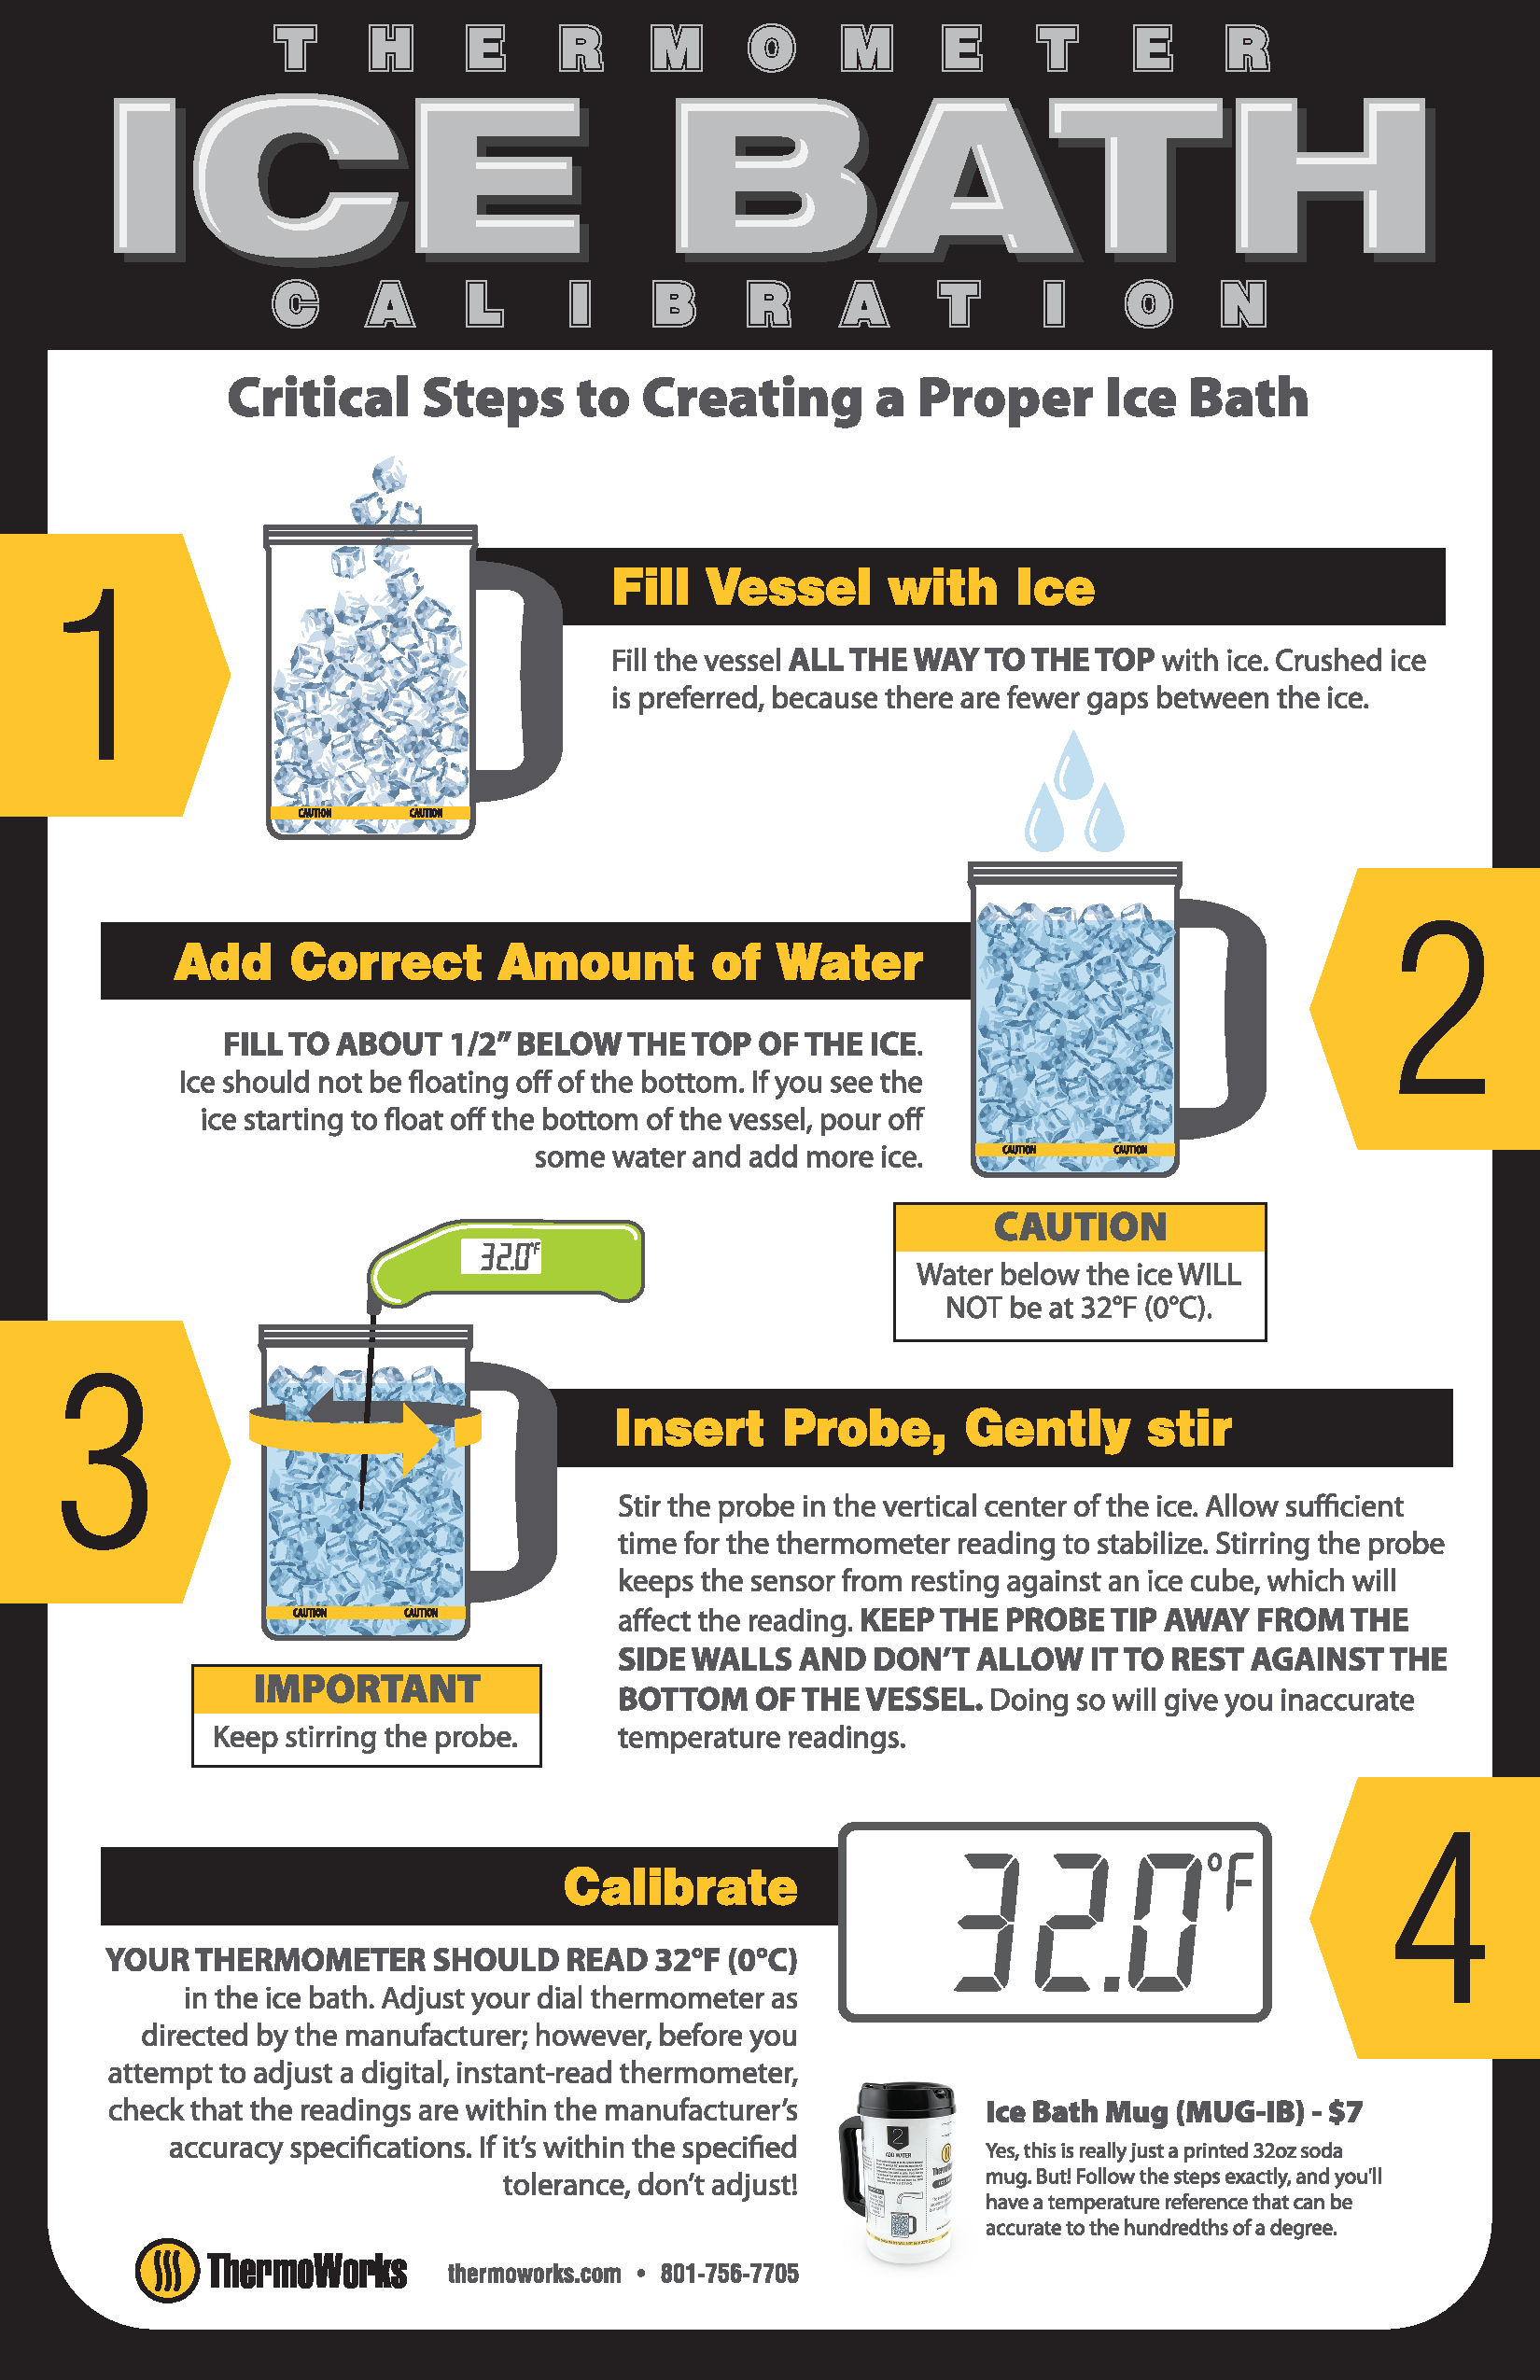
\includegraphics[height=0.85\textheight]{ref/ice_bath_infographic.pdf}
    \caption[Forma correcta de hacer un baño de hielo]{Forma correcta de hacer un baño de hielo}
    \label{fig:IceBath}
\end{figure}
\thispagestyle{formato-PI}
\renewcommand{\MayorVer}{2}
\renewcommand{\MenorVer}{0}
\renewcommand{\Titulo}{Mantenimiento de equipos de medición}
\renewcommand{\TipoID}{PRO}
\renewcommand{\FechaPub}{2023--01}

\section{\Titulo}\index{Programa!metrología, de}\index{Procedimiento!mantenimiento de termómetros}
\renewcommand{\Codigo}{\Prog--\thesection--\TipoID}

\subsection{Objetivo}

\begin{itemize}
	\item Garantizar que los valores de temperatura señalados por los equipos de medición indiquen valores reales y confiables para garantizar la calidad e inocuidad de los productos alimenticios recibidos, almacenados y distribuidos.
	\item Corrección de aquellos equipos que no cumplen los requerimientos establecidos.
\end{itemize}

\subsection{Alcance}
Aplica a los equipos de medición de las áreas operativas, termómetros de mano.

\subsection{Terminología y definiciones}
\begin{description}
    \defglo{metrologia}
    \defglo{proveedor}
\end{description}

\subsection{Procedimiento}
\subsubsection{Verificación externa}
\begin{itemize}
	\item \Gls{RDF} implementa un programa de calibración de sus equipos de medición por parte de una empresa externa calificada, la frecuencia se encuentra programada de manera anual.
	\item El \gls{proveedor} externo deberá presentar las certificaciones que lo acreditan como un proveedor certificado y contar con el suficiente entrenamiento para poder realizar los trabajos de calibración de los equipos.
	\item El servicio se llevará a cabo en las instalaciones del proveedor calificado.
	\item El prestador de servicios deberá entregar un informe de calibración (o certificado) por equipo y este a su vez será archivado como evidencia en la carpeta de registros.
	\item Si es necesaria una reparación, verificación o calibración intermedia a este programa, se llamará al proveedor de servicio para realizar el mantenimiento correspondiente.
    \item[NOTA:] Para revisar cualquier duda técnica, consulte el manual del usuario.
\item[NOTA:] Los termómetros colocados en cámaras solo se utilizan como referencia
\end{itemize}

\subsection{Responsables de la actividad}
\begin{itemize}
	\item \textbf{Ejecutado} por personal de mantenimiento;
	\item \textbf{Monitoreado} por personal de calidad;
	\item \textbf{Verificado} por personal de calidad.
\end{itemize}

\subsection{Frecuencia}
Anual

\begin{changelog}[simple, sectioncmd=\subsection*,label=changelog-\thesection-\MayorVer.\MenorVer]
	\begin{version}[v=\MayorVer.\MenorVer, date=2023--01, author=Pablo E. Alanis]
		\item Cambio de formato;
		\item Cambios en la serialización de versiones;
		\item Correcciones ortográficas y de estilo.
	\end{version}

	\begin{version}[v=1.7, date=2022--05, author=Alonso M.]
		\item cambio de fecha;
	\end{version}

	\shortversion{v=1.6, date=2021--05, changes=No hubo cambios}
\end{changelog}
\renewcommand{\MayorVer}{1}
\renewcommand{\MenorVer}{0}
\renewcommand{\TipoID}{G}
\renewcommand{\Codigo}{\Prog-\TipoID}
\renewcommand{\FechaPub}{2023--01}
%\renewcommand{\Edit}{01}
\renewcommand{\Titulo}{Programa de metrología --- Glosario}

\printunsrtglossary[type=acronym,nonumberlist]
\printunsrtglossary[type=\glsdefaulttype,nonumberlist]
% \printunsrtglossary[type=main]    
% \printglossary[type=acronym]
% \printglossary[type=main]
% \printunsrtglossary[type=acronym]
% \printunsrtglossary[type=main]
\renewcommand{\MayorVer}{1}
\renewcommand{\MenorVer}{0}
\renewcommand{\TipoID}{I}
\renewcommand{\Codigo}{\Prog-\TipoID}
\renewcommand{\FechaPub}{2023--01}
%\renewcommand{\Edit}{01}
\renewcommand{\Titulo}{Indice alfabético}
\printindex
\end{document}